\section{Extended partitioning: Select installation partitions}Select the partitions you want to use for installation and as swap space. You can only select partitions that can be used for installation or swap.\\
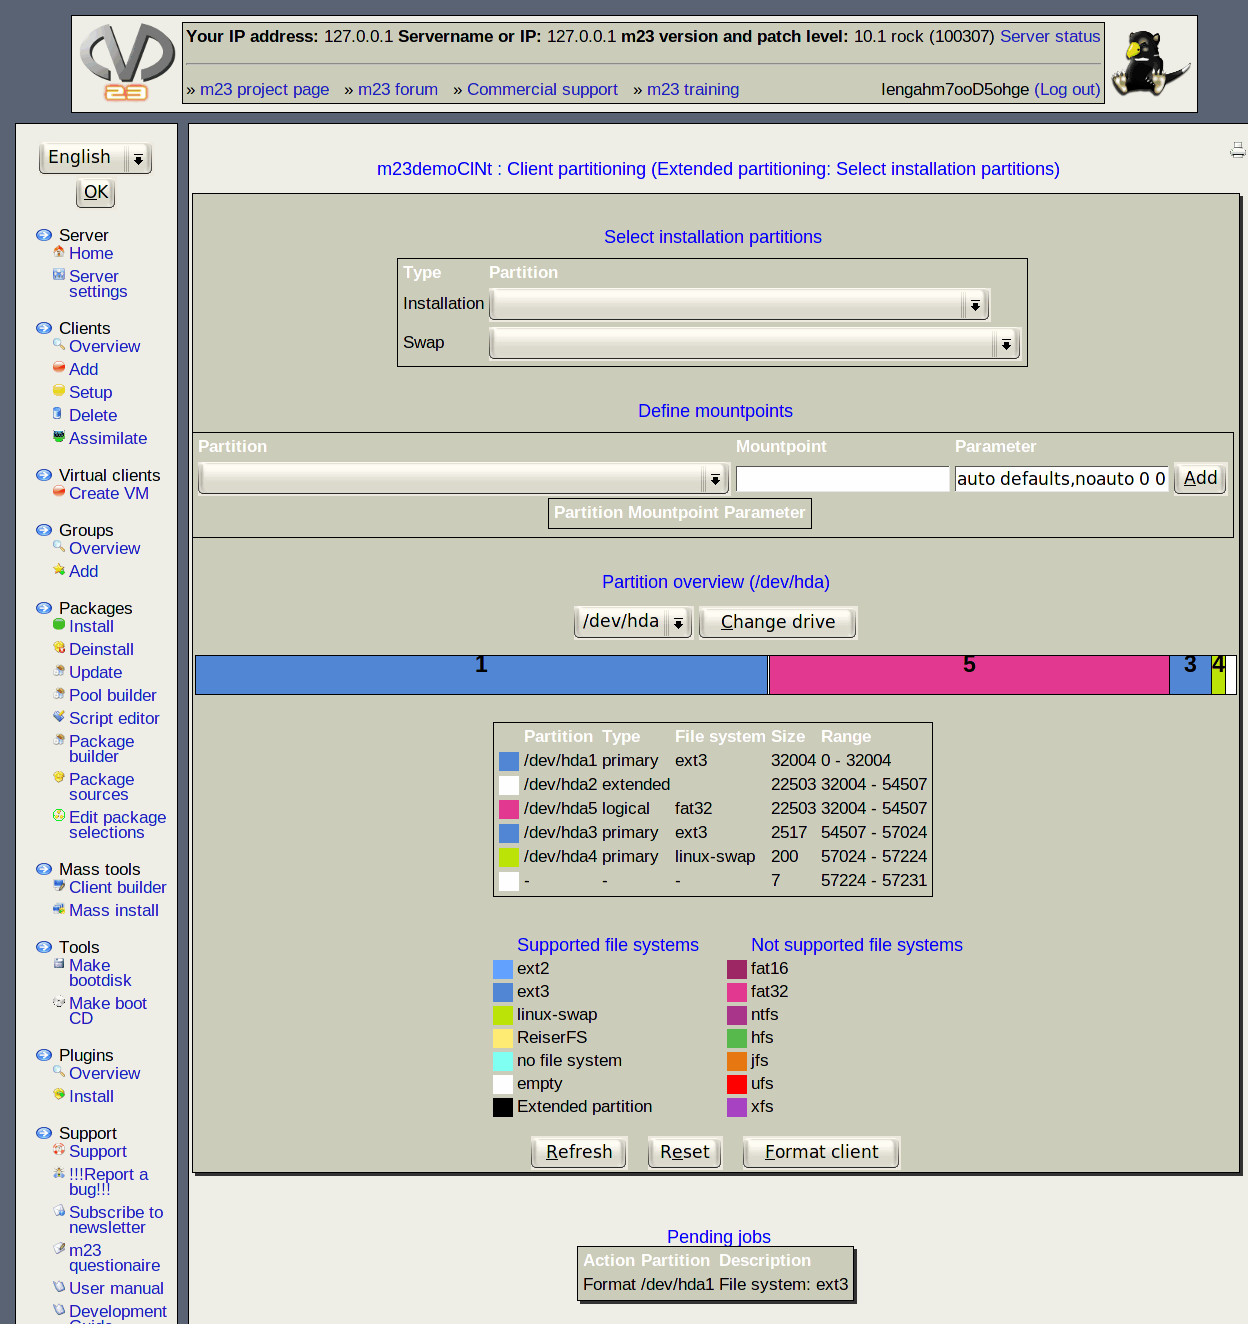
\includegraphics[scale=0.4]{/mdk/doc/manual/screenshots/en/fdisk-extended3.png} \\
\subsection{Step by step}
\begin{enumerate}
\item Choose the partitions for installation and as swap from the lists.\\
\item If you need additional mountpoints, you can define them under \textit{"Define mountpoints"}. Enter the partition, the mountpoint and the required parameters into the appropriate input fields and click on \textit{"Add"}. These informations correspond to those which you can find in the file \textbf{/etc/fstab}. You can see mountpoints which are already defined in the table under the input lines.\\
\item When you have made your selection, click on \textit{"Format client"}.\\
\end{enumerate}
\subsection{Hint for installation on a RAID}
You have to define a mountpoint, if you want to install an operating system on a RAID. Choose a partition which is not located on a RAID from the list \textit{"Partition"}. Enter \textbf{"/boot"} in \textit{"Mountpoint"} and \textbf{"auto defaults,noauto 0 0"} in \textit{"Parameter"}.\\
